\begin{enumerate}[label=\thechapter.\arabic*,ref=\thechapter.\theenumi]
\item Let a frequency modulated (FM) signal : $ x(t) = A \cos(\omega_c t + k_f \int_{-\infty}^{t} m(\lambda) d\lambda)$ , where $ m(t) $is a message signal of bandwidth $ W $. It is passed through a non-linear system with output $y(t) = 2x(t) + 5(x(t))^2 $.
Let $B_T $denote the FM bandwidth. The minimum value of $ \omega_c $ required to recover $ x(t) $ from $ y(t) $ is:\\
\begin{enumerate}[label = (\Alph*)]
\item $B_T + W$ \\
\item $\dfrac{3}{2} B_T$ \\
\item $2B_T + W$ \\
\item $\dfrac{5}{2} B_T$ \\
\end{enumerate}

\solution
\newpage

\item Let an input $x[n]$ having discrete-time Fourier transform
$X(e^{j\Omega}) = 1 - e^{-j\Omega} + 2e^{-3j\Omega}$
be passed through an LTI system. The frequency response of the LTI system is 
$H(e^{j\Omega}) = 1 - \frac{1}{2} e^{-2j\Omega}$
The output $y[n]$ of the system is \\ \hfill(GATE EC 2023)
\solution 
\input{2023/EC/48/ec48.tex}
\newpage
\item The Fourier transform $X(\omega)$ of $x(t) = e^{-t^2}$ is\\
Note:$\int_{-\infty}^{\infty} e^{-y^2} \,dy = \sqrt{\pi}$ \\  
A) $\sqrt{\pi} e^{\frac{\omega^2}{2}}$ \\
B) $\frac{e^{\frac{-\omega^2}{4}}}{2\sqrt{\pi}}$ \\
C) $\sqrt{\pi} e^{\frac{-\omega^2}{4}}$ \\
D) $\sqrt{\pi} e^{\frac{-\omega^2}{2}}$\\
\hfill Gate 2023 EC Question 28
\solution
\iffalse
\let\negmedspace\undefined
\let\negthickspace\undefined
\documentclass[journal,12pt,twocolumn]{IEEEtran}
\usepackage{cite}
\usepackage{amsmath,amssymb,amsfonts,amsthm}
\usepackage{algorithmic}
\usepackage{graphicx}
\usepackage{textcomp}
\usepackage{xcolor}
\usepackage{txfonts}
\usepackage{listings}
\usepackage{enumitem}
\usepackage{mathtools}
\usepackage{gensymb}
\usepackage{comment}
\usepackage[breaklinks=true]{hyperref}
\usepackage{tkz-euclide} 
\usepackage{listings}
\usepackage{gvv}                                        
\def\inputGnumericTable{}                                 
\usepackage[latin1]{inputenc}                                
\usepackage{color}                                            
\usepackage{array}                                            
\usepackage{longtable}                                       
\usepackage{calc}                                             
\usepackage{multirow}                                         
\usepackage{hhline}                                           
\usepackage{ifthen}                                           
\usepackage{lscape}


\newtheorem{theorem}{Theorem}[section]
\newtheorem{problem}{Problem}
\newtheorem{proposition}{Proposition}[section]
\newtheorem{lemma}{Lemma}[section]
\newtheorem{corollary}[theorem]{Corollary}
\newtheorem{example}{Example}[section]
\newtheorem{definition}[problem]{Definition}
\newcommand{\BEQA}{\begin{eqnarray}}
\newcommand{\EEQA}{\end{eqnarray}}
\newcommand{\define}{\stackrel{\triangle}{=}}
\theoremstyle{remark}
\newtheorem{rem}{Remark}
\begin{document}
\parindent 0px
\bibliographystyle{IEEEtran}

\title{Gate EE - 18}
\author{EE23BTECH11216 - P.kalyan$^{}$% <-this % stops a space
}
\maketitle
\newpage
\bigskip

\renewcommand{\thefigure}{\theenumi}
\renewcommand{\thetable}{\theenumi}
\section*{Question}
The Fourier transform x$\brak{\omega}$ of  the signal x\brak{t} is given by

\[
X(\omega) = 
\begin{cases} 
1, \text{for } |\omega| < \omega_0 \\
0, \text{for } |\omega| > \omega_0 
\end{cases}
\]

\text{(A) } x\brak{t} \text{ tends to be an impulse as } $W_0$ $\rightarrow \infty$.

\text{(B) } x\brak{0} \text{ decreases as } $W_0$ \text{ increases.}

\text{(C) At } t = $\frac{\pi}{2W_0}$, \quad x\brak{t} = -$\frac{1}{\pi}$.

\text{(D) At } t = $\frac{\pi}{2W_0}$, \quad x\brak{t} = $\frac{1}{\pi}$. \hfill\brak{\text{GATE EE 2023}}


 \fi

\begin{center}
    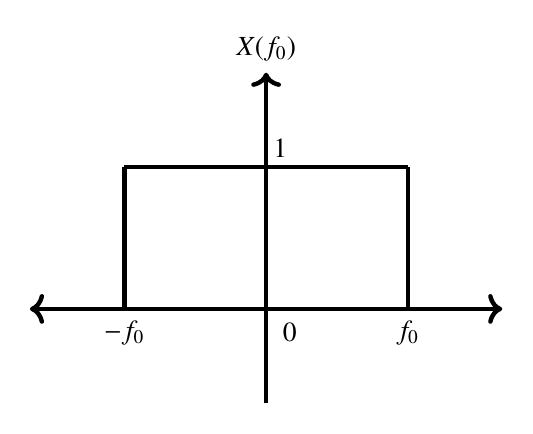
\begin{tikzpicture}[scale=0.6, ultra thick]
        \draw[->] (0,-2) -- (0,5);
        \draw (0,5.5) node {$X(f_{0}$)};
        \draw (0.5,-0.5)  node{0};
        \draw[<->]  (-5,0) -- (5,0);
        \draw  (3,3) -- (3,0);
        \draw (0.3,3.4) node{1};
        \draw (-3,3) -- (3,3);
        \draw (-3,3)--(-3,0);
        \draw (-3,-0.5) node {$-f_{0}$};

        \draw (3,-0.5) node {$f_{0}$};
    \end{tikzpicture}
\end{center}

By taking inverse Fourier transform,
\begin{align}
x\brak{t} = \frac{\sin\brak{ t}}{\pi t}
\end{align}

\begin{align}
& x\left(\frac{\pi}{2\brak{2\pi f_{0}}}\right) =\frac{2 \brak{2\pi f_{0}}}{\pi^2}
\end{align}

So, option \brak{C} and \brak{D} are wrong.

\begin{align}
x\brak{0}=\lim_{t\to 0}\frac{\sin \brak{2\pi f_{0}} t}{\pi t}=\frac{2\pi f_{0}}{\pi}
\end{align}

So, $x\brak{0} \propto f_{0} \Rightarrow$ Option \brak{B} is wrong.\\

When $f_{0}\rightarrow \infty$, $X\brak{f_{0}}$ will be a D.C signal and inverse Fourier transform of a D.C signal will be impulse signal\\[3ex]
So, option \brak{A} is correct
\begin{figure}[ht]
    \centering
    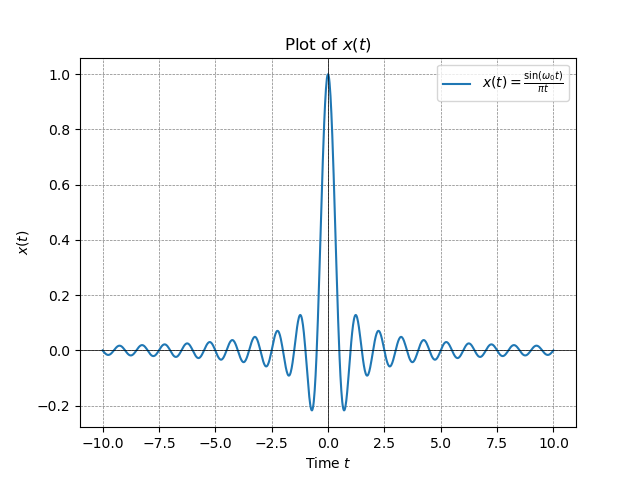
\includegraphics[width=1\columnwidth]{2023/EE/18/figs/main.png}
    \caption{plot of X\brak{t}}
    \label{fig:EE18.1}
\end{figure}


\newpage

 \item Let $x(t) = 10 \cos(10.5 \omega t)$ be passed through an LTI system with impulse response $h(t) = \pi\left(\frac{\sin(\omega t)}{\pi t}\right)^2 \cos(10 \omega t)$ . The output of the system is:\\ \hfill(GATE EC 2023)\\
A) $\frac{15}{4}\omega \cos(10.5 \omega t)$ \\
B) $\frac{15}{2}\omega \cos(10.5 \omega t)$ \\
C) $\frac{15}{8}\omega \cos(10.5 \omega t)$ \\
D) $15\omega \cos(10.5 \omega t)$ \\
 \solution
\iffalse
\let\negmedspace\undefined
\let\negthickspace\undefined
\documentclass[journal,12pt,onecolumn]{IEEEtran}
\usepackage{cite}
\usepackage{amsmath,amssymb,amsfonts,amsthm}
\usepackage{algorithmic}
\usepackage{graphicx}
\usepackage{textcomp}
\usepackage{xcolor}
\usepackage{multirow}
\usepackage{txfonts}
\usepackage{listings}
\usepackage{enumitem}
\usepackage{mathtools}
\usepackage{gensymb}

\usepackage{tkz-euclide} % loads  TikZ and tkz-base
\usepackage{listings}



\newtheorem{theorem}{Theorem}[section]
\newtheorem{problem}{Problem}
\newtheorem{proposition}{Proposition}[section]
\newtheorem{lemma}{Lemma}[section]
\newtheorem{corollary}[theorem]{Corollary}
\newtheorem{example}{Example}[section]
\newtheorem{definition}[problem]{Definition}
%\newtheorem{thm}{Theorem}[section] 
%\newtheorem{defn}[thm]{Definition}
%\newtheorem{algorithm}{Algorithm}[section]
%\newtheorem{cor}{Corollary}
\newcommand{\BEQA}{\begin{eqnarray}}
\newcommand{\EEQA}{\end{eqnarray}}
\newcommand{\system}[1]{\stackrel{#1}{\rightarrow}}

\newcommand{\define}{\stackrel{\triangle}{=}}
\theoremstyle{remark}
\newtheorem{rem}{Remark}
%\bibliographystyle{ieeetr}
\begin{document}
%
\providecommand{\pr}[1]{\ensuremath{\Pr\left(#1\right)}}
\providecommand{\prt}[2]{\ensuremath{p_{#1}^{\left(#2\right)} }}        % own macro for this question
\providecommand{\qfunc}[1]{\ensuremath{Q\left(#1\right)}}
\providecommand{\sbrak}[1]{\ensuremath{{}\left[#1\right]}}
\providecommand{\lsbrak}[1]{\ensuremath{{}\left[#1\right.}}
\providecommand{\rsbrak}[1]{\ensuremath{{}\left.#1\right]}}
\providecommand{\brak}[1]{\ensuremath{\left(#1\right)}}
\providecommand{\lbrak}[1]{\ensuremath{\left(#1\right.}}
\providecommand{\rbrak}[1]{\ensuremath{\left.#1\right)}}
\providecommand{\cbrak}[1]{\ensuremath{\left\{#1\right\}}}
\providecommand{\lcbrak}[1]{\ensuremath{\left\{#1\right.}}
\providecommand{\rcbrak}[1]{\ensuremath{\left.#1\right\}}}
\newcommand{\sgn}{\mathop{\mathrm{sgn}}}
\providecommand{\abs}[1]{\left\vert#1\right\vert}
\providecommand{\res}[1]{\Res\displaylimits_{#1}} 
\providecommand{\norm}[1]{\left\lVert#1\right\rVert}
%\providecommand{\norm}[1]{\lVert#1\rVert}
\providecommand{\mtx}[1]{\mathbf{#1}}
\providecommand{\mean}[1]{E\left[ #1 \right]}
\providecommand{\cond}[2]{#1\middle|#2}
\providecommand{\fourier}{\overset{\mathcal{F}}{ \rightleftharpoons}}
\newenvironment{amatrix}[1]{%
  \left(\begin{array}{@{}*{#1}{c}|c@{}}
}{%
  \end{array}\right)
}
%\providecommand{\hilbert}{\overset{\mathcal{H}}{ \rightleftharpoons}}
%\providecommand{\system}{\overset{\mathcal{H}}{ \longleftrightarrow}}
	%\newcommand{\solution}[2]{\textbf{Solution:}{#1}}
\newcommand{\solution}{\noindent \textbf{Solution: }}
\newcommand{\cosec}{\,\text{cosec}\,}
\providecommand{\dec}[2]{\ensuremath{\overset{#1}{\underset{#2}{\gtrless}}}}
\newcommand{\myvec}[1]{\ensuremath{\begin{pmatrix}#1\end{pmatrix}}}
\newcommand{\mydet}[1]{\ensuremath{\begin{vmatrix}#1\end{vmatrix}}}
\newcommand{\myaugvec}[2]{\ensuremath{\begin{amatrix}{#1}#2\end{amatrix}}}
\providecommand{\rank}{\text{rank}}
\providecommand{\pr}[1]{\ensuremath{\Pr\left(#1\right)}}
\providecommand{\qfunc}[1]{\ensuremath{Q\left(#1\right)}}
	\newcommand*{\permcomb}[4][0mu]{{{}^{#3}\mkern#1#2_{#4}}}
\newcommand*{\perm}[1][-3mu]{\permcomb[#1]{P}}
\newcommand*{\comb}[1][-1mu]{\permcomb[#1]{C}}
\providecommand{\qfunc}[1]{\ensuremath{Q\left(#1\right)}}
\providecommand{\gauss}[2]{\mathcal{N}\ensuremath{\left(#1,#2\right)}}
\providecommand{\diff}[2]{\ensuremath{\frac{d{#1}}{d{#2}}}}
\providecommand{\myceil}[1]{\left \lceil #1 \right \rceil }
\newcommand\figref{Fig.~\ref}
\newcommand\tabref{Table~\ref}
\newcommand{\sinc}{\,\text{sinc}\,}
\newcommand{\rect}{\,\text{rect}\,}
%%
%	%\newcommand{\solution}[2]{\textbf{Solution:}{#1}}
%\newcommand{\solution}{\noindent \textbf{Solution: }}
%\newcommand{\cosec}{\,\text{cosec}\,}
%\numberwithin{equation}{section}
%\numberwithin{equation}{subsection}
%\numberwithin{problem}{section}
%\numberwithin{definition}{section}
%\makeatletter
%\@addtoreset{figure}{problem}
%\makeatother

%\let\StandardTheFigure\thefigure
\let\vec\mathbf

\bibliographystyle{IEEEtran}





\bigskip



\title{GATE ECE 2023}
\author{Karyampudi Meghana Sai\\ EE23BTECH11031}
\maketitle
Consider a discrete-time signal with period $N=5$. Let the discrete-time Fourier series (DTFS) representation be $x[n]=\sum\limits_{k=0}^{4} a_k e^{\frac{jk2\pi n}{5}}$, where $a_0=1$, $a_1=3j$, $a_2=2j$, $a_3=-2j$, $a_4=-3j$. The value of the sum $\sum\limits_{n=0}^{4}x[n] \sin\brak{\frac{4\pi n}{5}}$ is\\
(A) -10\\
(B) 10\\
(C) -2\\
(D) 2\\
\hfill Gate 2023 EC 47

\solution\\
\fi
\begin{enumerate}
\item Solving the question for N=5:
\begin{table}[h!]
 	\centering
 	\resizebox{6 cm}{!}{
 		\begin{tabular}{|c|c|c|}
    \hline
    \textbf{Parameter} & \textbf{Value} & \textbf{Description} \\[6pt]
    \hline
    $N$ &  $5$ & Time period \\ \cline{1-2}\cline{3-3}
    $X(k)$ & $\sum\limits_{n=0}^{N-1} x(n)e^{\frac{-j2\pi kn}{N}}$ & DFT formula\\ \cline{1-2}\cline{3-3}
    $X(0)$ &  $5$ & \multirow{5}{*}{\begin{tabular}[c]{@{}c@{}}DFT\\ values\end{tabular}} \\ \cline{1-2}
    $X(1)$ &  $15j$ &    \\ \cline{1-2}
    $X(2)$ &  $10j$ &    \\ \cline{1-2}
    $X(3)$ &  $-10j$ &    \\ \cline{1-2}
    $X(4)$ &  $-15j$ &    \\ \hline 
\end{tabular}

 	}
 	\vspace{6 pt}
 	\caption{Input Parameters}
 	\label{tab:gate23ec47tab2}
 \end{table} 
\begin{align}
\sum\limits_{n=0}^{4}x(n) \sin\brak{\frac{4\pi n}{5}}&=\sum\limits_{n=0}^{4}x(n)\sbrak{\frac{e^{\frac{j4\pi n}{5}}-e^{\frac{-j4\pi n}{5}}}{2j}}\\
&=\frac{1}{2j}\sbrak{\sum\limits_{n=0}^{4}x(n)e^{\frac{j2\pi (2)n}{5}}-\sum\limits_{n=0}^{4}x(n)e^{\frac{-j2\pi (2)n}{5}}}\label{eq:gate23ec47eq2}
\end{align}

Refering to the table \ref{tab:gate23ec47tab2}.\\
\begin{align}
X(k)&=\sum\limits_{n=0}^{4} x(n)e^{\frac{-j2\pi kn}{5}}\label{eq:gate23ec47eq3}
\end{align}
Referencing from equation \eqref{eq:gate23ec47eq3}, equation \eqref{eq:gate23ec47eq2} can be written as:
\begin{align}
\sum\limits_{n=0}^{4}x(n) \sin\brak{\frac{4\pi n}{5}}&=\frac{1}{2j}\sbrak{X(-2)-X(2)}\label{eq:gate23ec47eq4}
\end{align}
From the property of discrete Fourier series.\\
\begin{align}
X(k)=X(k+N)
\end{align}
So, equation \eqref{eq:gate23ec47eq4} becomes,\\
\begin{align}
\sum\limits_{n=0}^{4}x(n) \sin\brak{\frac{4\pi n}{5}}&=\frac{1}{2j}\sbrak{X(3)-X(2)}\\
\sum\limits_{n=0}^{4}x(n) \sin\brak{\frac{4\pi n}{5}}&=-10
\end{align}
\begin{figure}[htbp]
    \centering
    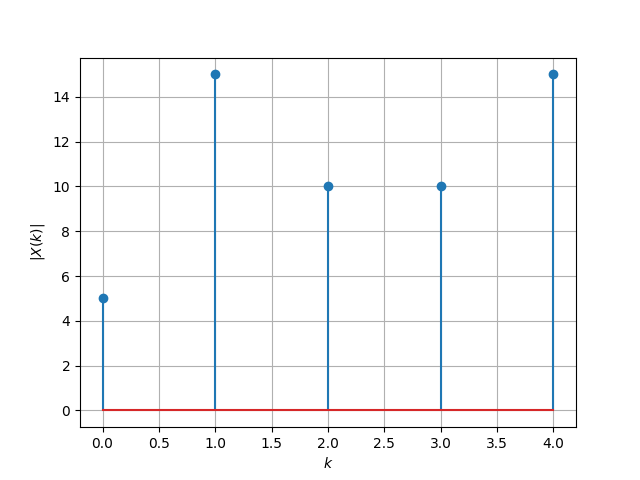
\includegraphics[width=\columnwidth]{2023/EC/47/figs/mm1.png}
    \caption{Amplitude of equation \eqref{eq:gate23ec47eq3}}
    \label{fig:gate23ec47fig1}
\end{figure}
\begin{figure}[htbp]
    \centering
    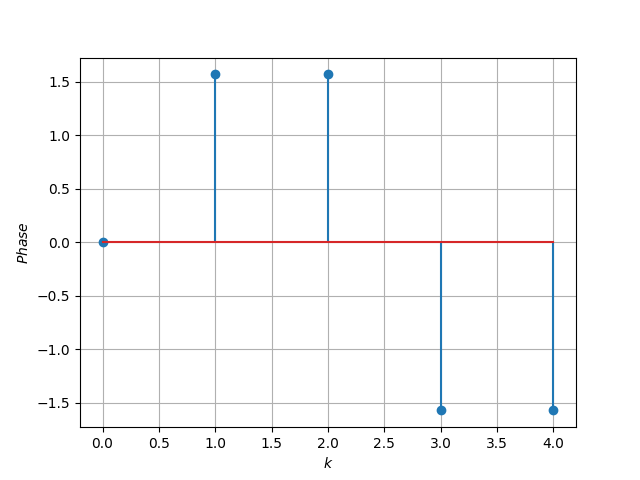
\includegraphics[width=\columnwidth]{2023/EC/47/figs/mm11.png}
    \caption{Phase of equation \eqref{eq:gate23ec47eq3}}
    \label{fig:gate23ec47fig2}
\end{figure}

\item Solving the question for N=8:
\begin{table}[h!]
 	\centering
 	\resizebox{6 cm}{!}{
 		\begin{tabular}{|c|c|c|}
    \hline
    \textbf{Parameter} & \textbf{Value} & \textbf{Description} \\[6pt]
    \hline
    $N$ &  $8$ & Time period \\ \cline{1-2}\cline{3-3}
    $X(k)$ &  $\sum\limits_{n=0}^{N-1} x(n)e^{\frac{-j2\pi kn}{N}}$ & DFT formula\\ \cline{1-2}\cline{3-3}
    $X(0)$ &  $8$ & \multirow{5}{*}{\begin{tabular}[c]{@{}c@{}}DFT \\ values\end{tabular}} \\ \cline{1-2}
    $X(1)$ &  $24j$ &    \\ \cline{1-2}
    $X(2)$ &  $16j$ &    \\ \cline{1-2}
    $X(3)$ &  $-16j$ &    \\ \cline{1-2}
    $X(4)$ &  $-24j$ &    \\ \cline{1-2}
    $X(5)$ &  $0$ &    \\ \cline{1-2}
    $X(6)$ &  $0$ &    \\ \cline{1-2}
    $X(7)$ &  $0$ &    \\ \hline
\end{tabular}

 	}
 	\vspace{6 pt}
 	\caption{Input Parameters}
 	\label{tab:gate23ec47tab1}
 \end{table} 
\begin{align}
\sum\limits_{n=0}^{7}x(n) \sin\brak{\frac{4\pi n}{8}}&=\sum\limits_{n=0}^{7}x(n)\sbrak{\frac{e^{\frac{j4\pi n}{8}}-e^{\frac{-j4\pi n}{8}}}{2j}}\\
&=\frac{1}{2j}\sbrak{\sum\limits_{n=0}^{7}x(n)e^{\frac{j2\pi (2)n}{8}}-\sum\limits_{n=0}^{7}x(n)e^{\frac{-j2\pi (2)n}{8}}}\label{eq:gate23ec47eq9}
\end{align}

Refering to the table \ref{tab:gate23ec47tab1}.
\begin{align}
X(k)&=\sum\limits_{n=0}^{7} x(n)e^{\frac{-j2\pi kn}{8}}\label{eq:gate23ec47eq10}
\end{align}
Referencing from equation\eqref{eq:gate23ec47eq10}, equation\eqref{eq:gate23ec47eq9} can be written as:
\begin{align}
\sum\limits_{n=0}^{7}x(n) \sin\brak{\frac{4\pi n}{8}}&=\frac{1}{2j}\sbrak{X(-2)-X(2)}\label{eq:gate23ec47eq11}
\end{align}
From the property of discrete Fourier series.\\
\begin{align}
X(k)=X(k+N)
\end{align}
So, equation\eqref{eq:gate23ec47eq11} becomes,\\
\begin{align}
\sum\limits_{n=0}^{7}x(n) \sin\brak{\frac{4\pi n}{8}}&=\frac{1}{2j}\sbrak{X(6)-X(2)}\\
\sum\limits_{n=0}^{7}x(n) \sin\brak{\frac{4\pi n}{8}}&=-8
\end{align}
\begin{figure}[h!]
    \centering
    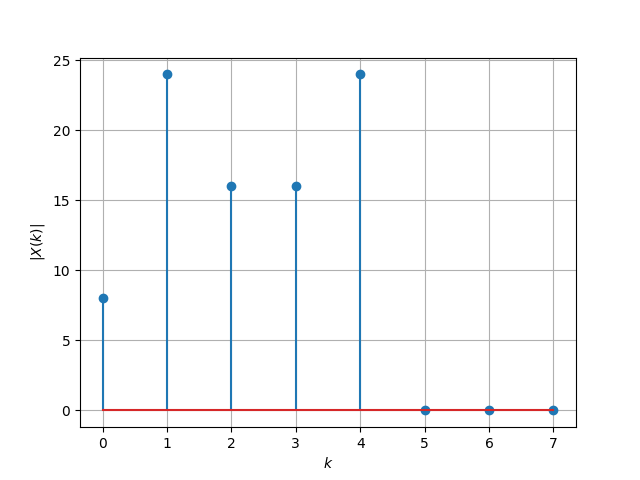
\includegraphics[width=\columnwidth]{2023/EC/47/figs/mm2.png}
    \caption{Amplitude of equation \eqref{eq:gate23ec47eq10}}
    \label{fig:gate23ec47fig3}
\end{figure}
\begin{figure}[h!]
    \centering
    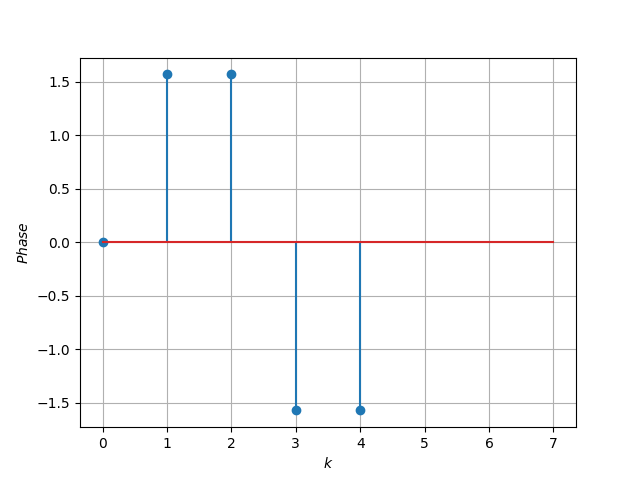
\includegraphics[width=\columnwidth]{2023/EC/47/figs/mm21.png}
    \caption{Phase of equation \eqref{eq:gate23ec47eq10}}
    \label{fig:gate23ec47fig4}
\end{figure}

\end{enumerate}

%\end{document}

\newpage
 
 \item Q27) Let m\brak{\text{t}} be a strictly band-limited signal with bandwidth B and energy E. Assuming $\omega_0$ = 10B, the energy in the signal $\text{m}\brak{\text{t}}\text{cos}\brak{\omega_0\text{t}}$\\[1ex]
\brak{\text{A}}\ $\frac{\text{E}}{4}$\\[1ex]
\brak{\text{B}}\ $\frac{\text{E}}{2}$\\[1ex]
\brak{\text{C}}\ \text{E}\\[1ex]
\brak{\text{D}}\ 2\text{E} \qquad\qquad\qquad\quad\qquad\qquad\qquad\qquad\brak{\text{GATE EC 2023}}

\solution
\input{2023/EC/27/gate,2k23.tex}
\newpage

\item The following function is defined over the interval $[-L,L]:$
    $$f\brak{x}=px^4+qx^5$$
It is expressed as a Fourier series,
    $$f\brak{x}=a\brak{0}+\sum_{n=1}^{\infty}\cbrak{a\brak{n}\sin\brak{\frac{\pi x}{L}}+b\brak{n}\cos\brak{\frac{\pi x}{L}}}$$

which options amongst the following are true?
\begin{enumerate}[label=(\alph*)]
    \item $a\brak{n}$, $n=1,2,..,\infty$ depend on $p$
    \item $a\brak{n}$, $n=1,2,..,\infty$ depend on $q$
    \item $b\brak{n}$, $n=1,2,..,\infty$ depend on $p$
    \item $b\brak{n}$, $n=1,2,..,\infty$ depend on $q$
\end{enumerate}
\hfill(GATE 2023 CE Question 25)\\
\solution
\iffalse
\let\negmedspace\undefined
\let\negthickspace\undefined
\documentclass[journal,12pt,twocolumn]{IEEEtran}
\usepackage{cite}
\usepackage{amsmath,amssymb,amsfonts,amsthm}
\usepackage{algorithmic}
\usepackage{graphicx}
\usepackage{textcomp}
\usepackage{xcolor}
\usepackage{txfonts}
\usepackage{listings}
\usepackage{enumitem}
\usepackage{mathtools}
\usepackage{gensymb}
\usepackage{comment}
\usepackage[breaklinks=true]{adjustbox}
\usepackage{tkz-euclide} 
\usepackage{listings}
\usepackage{gvv}                                        
\def\inputGnumericTable{}                                 
\usepackage[latin1]{inputenc}                                
\usepackage{color}                                            
\usepackage{array}                                            
\usepackage{longtable}                                       
\usepackage{calc}                                             
\usepackage{multirow}                                         
\usepackage{hhline}                                           
\usepackage{ifthen}                                           
\usepackage{lscape}

\newtheorem{theorem}{Theorem}[section]
\newtheorem{problem}{Problem}
\newtheorem{proposition}{Proposition}[section]
\newtheorem{lemma}{Lemma}[section]
\newtheorem{corollary}[theorem]{Corollary}
\newtheorem{example}{Example}[section]
\newtheorem{definition}[problem]{Definition}
\newcommand{\BEQA}{\begin{eqnarray}}
\newcommand{\EEQA}{\end{eqnarray}}
\newcommand{\define}{\stackrel{\triangle}{=}}
\theoremstyle{remark}
\newtheorem{rem}{Remark}

\begin{document}
\bibliographystyle{IEEEtran}

\vspace{3cm}

\title{}
\author{EE23BTECH11024 - G.Karthik Yadav$^{*}$
}
\maketitle
\newpage
\bigskip

\section*{GATE 2023 EC 41}
\noindent 1. \hspace{2pt} A Closed loop systen is shown in the figure where $k>0$ and $\alpha>0$ .\\
The Steady State error due to a ramp input $\brak{R\brak{s} = \alpha s^{-2}}$ is given by \hfill{(GATE 2023 EC 41)}

\begin{figure}[ht]
\centering
    \includegraphics[width=1.0\linewidth]{2023/EC/41/figs/question.png}
    \label{fig: 23.EC.41.24.1}
\end{figure}

\begin{enumerate}
\item $\frac{2\alpha}{k}$
\item $\frac{\alpha}{k}$
\item $\frac{\alpha}{2k}$
\item $\frac{\alpha}{4k}$
\end{enumerate}

\solution\\
\fi
\begin{table}[ht]
\setlength{\arrayrulewidth}{0.3mm}
\setlength{\tabcolsep}{15pt}
\renewcommand{\arraystretch}{1.5}



\begin{tabular}{ |p{1cm}|p{3cm}|p{1cm}| }
\hline
Symbol & Parameters & Value\\
\hline
$R\brak{s}$ & Laplace transform Ramp input signal r\brak{t} &  $\alpha s^{-2}$\\
\hline
$G\brak{s}$ & Open Loop transfer function &  $ \frac{Y\brak{s}}{E\brak{s}} = \frac{k}{s\brak{s+2}}$\\
\hline
$Y\brak{s}$ & Laplace transform of the output signal y\brak{t}  &  ? \\
\hline
$E\brak{s}$ & Laplace transform of the error signal e\brak{t} & R\brak{s} - Y\brak{s}\\
\hline
$E\brak{s}$ & Laplace transform of the error signal e\brak{t} & R\brak{s} - Y\brak{s}\\   
\hline
$e_s$ & Steady State Error &  ? \\
\hline
%$x(l)$ & Last($l^{th}$) term of series & 350\\
%$x(0)$ & Starting ($0^{th}$) term of series & 17 %\\
%\hline
%d & Common difference of AP & 9\\
%\hline
\end{tabular}
\caption{Parameters}






\end{table}
\bigskip
from table  Open loop transfer function $G\brak{s}$\\
\begin{align}
	G\brak{s} &= \frac{Y\brak{s}}{E\brak{s}} \label{24.2023.EC.41.1} \\
        &= \frac{Y\brak{s}}{R\brak{s} - Y\brak{s}} \\
        Y\brak{s} &= \frac{R\brak{s}G\brak{s}}{1 + G\brak{s}} \label{24.2023.EC.41.2}
\end{align}

from eq \ref{24.2023.EC.41.1} and eq \eqref{24.2023.EC.41.2}

\begin{align}
        G\brak{s} &= \frac{k}{s\brak{s +2}}  \label{24.2023.EC.41.3} \\ 
        Y\brak{s} &= \frac{\alpha k s^{-2}}{k + s\brak{s+2}} \label{24.2023.EC.41.4} \\
        E\brak{s} &= R\brak{s} - Y\brak{s}  \label{24.2023.EC.41.5} \\ 
        E\brak{s} &= \frac{\alpha \brak{s+2}}{s\brak{k + s\brak{s+2}}}
\end{align}

By Taking Inverse Laplace Transform of eq \eqref{24.2023.EC.41.3} and eq\eqref{24.2023.EC.41.4}

\begin{align}
    g\brak{t} &= \frac{k\brak{1 - e^{-2t}}}{2} u\brak{t} \\
        y\brak{t} &= \alpha t u\brak{t}- \frac{2\alpha}{k}u\brak{t} \\
        \notag &+\frac{\alpha}{2k\sqrt{1-k}} \biggl(2\sqrt{1-k}e^{\sqrt{1-k}t-1}\\ 
        \notag &+ 2\sqrt{1-k}e^{-\sqrt{1-k}t-1} \\
        \notag &+ \brak{2-k}e^{\sqrt{1-k}t-1} - \brak{2-k}e^{-\sqrt{1-k}t-1} \biggr) u\brak{t}
\end{align}

\begin{align}
        e\brak{t} &= r\brak{t} - y\brak{t} \\
        &= \alpha t u\brak{t} - y\brak{t} \\
        e\brak{t} &= \frac{2\alpha}{k}u\brak{t} \\
        \notag &-\frac{\alpha}{2k\sqrt{1-k}} \biggl(2\sqrt{1-k}e^{\sqrt{1-k}t-1}\\ 
        \notag &+ 2\sqrt{1-k}e^{-\sqrt{1-k}t-1} \\
        \notag &+ \brak{2-k}e^{\sqrt{1-k}t-1} - \brak{2-k}e^{-\sqrt{1-k}t-1} \biggr) u\brak{t}
\end{align}
	

\begin{align}
    e_s &= \displaystyle\lim_{s\to 0}s E\brak{s} \\
    &= \displaystyle\lim_{s\to 0} s \frac{R\brak{s}}{1 + G\brak{s}} \\
    &= \displaystyle\lim_{s\to 0} \frac{\alpha \brak{s+2}}{s\brak{s+2} + k} \\
    e_s &= \frac{2\alpha}{k}
\end{align}



\newpage
\item A continuous real-valued signal $x\brak{t}$ has finite positive energy and $x\brak{t} = 0$, $\forall$ $t < 0$. From the list given below, select ALL the signals whose
continuous-time Fourier transform is purely imaginary.\\
\begin{enumerate}
\item$x\brak{t} + x\brak{-t}$
\item$x\brak{t} - x\brak{-t}$
\item$j\brak{x\brak{t} + x\brak{-t}}$
\item$j\brak{x\brak{t} - x\brak{-t}}$
\end{enumerate}
\hfill{(GATE IN 2023)}\\
\solution
\input{2023/IN/44/Gate.tex}
\item Let $x_1(t) = u(t + 1.5) - u(t - 1.5)$ and $x_2(t)$ is shown in the figure below. For $y(t) = x_1(t) * x_2(t)$, the $\int_{-\infty}^{\infty} y(t) \, dt$ is \underline{\hspace{2cm}}.\\

\begin{figure}[htbp]
    \centering
    \includegraphics[width=0.5\textwidth]{2023/EC/58/figs/gatefig.png}
    \caption{Figure}
    \label{fig:graph}
\end{figure}

\hfill{(GATE IN 2023)}\\
\solution
\input{2023/EC/58/gate_ec_58.tex}
\pagebreak
\item Consider a discrete-time signal with period $N=5$. Let the discrete-time Fourier series (DTFS) representation be $ x[n] = \sum\limits_{k=0}^{4} a_k e^{\frac{jk2\pi n}{5}} $where $a_0=1$, $a_1=3j$, $a_2=2j$, $a_3=-2j$, $a_4=-3j$. The value of the sum $\sum\limits_{n=0}^{4}x[n] \sin\left(\frac{4\pi n}{5}\right) $is\\
(A) -10\\
(B) 10\\
(C) -2\\
(D) 2\\
\hfill Gate 2023 EC 47
\solution
\iffalse
\let\negmedspace\undefined
\let\negthickspace\undefined
\documentclass[journal,12pt,onecolumn]{IEEEtran}
\usepackage{cite}
\usepackage{amsmath,amssymb,amsfonts,amsthm}
\usepackage{algorithmic}
\usepackage{graphicx}
\usepackage{textcomp}
\usepackage{xcolor}
\usepackage{multirow}
\usepackage{txfonts}
\usepackage{listings}
\usepackage{enumitem}
\usepackage{mathtools}
\usepackage{gensymb}

\usepackage{tkz-euclide} % loads  TikZ and tkz-base
\usepackage{listings}



\newtheorem{theorem}{Theorem}[section]
\newtheorem{problem}{Problem}
\newtheorem{proposition}{Proposition}[section]
\newtheorem{lemma}{Lemma}[section]
\newtheorem{corollary}[theorem]{Corollary}
\newtheorem{example}{Example}[section]
\newtheorem{definition}[problem]{Definition}
%\newtheorem{thm}{Theorem}[section] 
%\newtheorem{defn}[thm]{Definition}
%\newtheorem{algorithm}{Algorithm}[section]
%\newtheorem{cor}{Corollary}
\newcommand{\BEQA}{\begin{eqnarray}}
\newcommand{\EEQA}{\end{eqnarray}}
\newcommand{\system}[1]{\stackrel{#1}{\rightarrow}}

\newcommand{\define}{\stackrel{\triangle}{=}}
\theoremstyle{remark}
\newtheorem{rem}{Remark}
%\bibliographystyle{ieeetr}
\begin{document}
%
\providecommand{\pr}[1]{\ensuremath{\Pr\left(#1\right)}}
\providecommand{\prt}[2]{\ensuremath{p_{#1}^{\left(#2\right)} }}        % own macro for this question
\providecommand{\qfunc}[1]{\ensuremath{Q\left(#1\right)}}
\providecommand{\sbrak}[1]{\ensuremath{{}\left[#1\right]}}
\providecommand{\lsbrak}[1]{\ensuremath{{}\left[#1\right.}}
\providecommand{\rsbrak}[1]{\ensuremath{{}\left.#1\right]}}
\providecommand{\brak}[1]{\ensuremath{\left(#1\right)}}
\providecommand{\lbrak}[1]{\ensuremath{\left(#1\right.}}
\providecommand{\rbrak}[1]{\ensuremath{\left.#1\right)}}
\providecommand{\cbrak}[1]{\ensuremath{\left\{#1\right\}}}
\providecommand{\lcbrak}[1]{\ensuremath{\left\{#1\right.}}
\providecommand{\rcbrak}[1]{\ensuremath{\left.#1\right\}}}
\newcommand{\sgn}{\mathop{\mathrm{sgn}}}
\providecommand{\abs}[1]{\left\vert#1\right\vert}
\providecommand{\res}[1]{\Res\displaylimits_{#1}} 
\providecommand{\norm}[1]{\left\lVert#1\right\rVert}
%\providecommand{\norm}[1]{\lVert#1\rVert}
\providecommand{\mtx}[1]{\mathbf{#1}}
\providecommand{\mean}[1]{E\left[ #1 \right]}
\providecommand{\cond}[2]{#1\middle|#2}
\providecommand{\fourier}{\overset{\mathcal{F}}{ \rightleftharpoons}}
\newenvironment{amatrix}[1]{%
  \left(\begin{array}{@{}*{#1}{c}|c@{}}
}{%
  \end{array}\right)
}
%\providecommand{\hilbert}{\overset{\mathcal{H}}{ \rightleftharpoons}}
%\providecommand{\system}{\overset{\mathcal{H}}{ \longleftrightarrow}}
	%\newcommand{\solution}[2]{\textbf{Solution:}{#1}}
\newcommand{\solution}{\noindent \textbf{Solution: }}
\newcommand{\cosec}{\,\text{cosec}\,}
\providecommand{\dec}[2]{\ensuremath{\overset{#1}{\underset{#2}{\gtrless}}}}
\newcommand{\myvec}[1]{\ensuremath{\begin{pmatrix}#1\end{pmatrix}}}
\newcommand{\mydet}[1]{\ensuremath{\begin{vmatrix}#1\end{vmatrix}}}
\newcommand{\myaugvec}[2]{\ensuremath{\begin{amatrix}{#1}#2\end{amatrix}}}
\providecommand{\rank}{\text{rank}}
\providecommand{\pr}[1]{\ensuremath{\Pr\left(#1\right)}}
\providecommand{\qfunc}[1]{\ensuremath{Q\left(#1\right)}}
	\newcommand*{\permcomb}[4][0mu]{{{}^{#3}\mkern#1#2_{#4}}}
\newcommand*{\perm}[1][-3mu]{\permcomb[#1]{P}}
\newcommand*{\comb}[1][-1mu]{\permcomb[#1]{C}}
\providecommand{\qfunc}[1]{\ensuremath{Q\left(#1\right)}}
\providecommand{\gauss}[2]{\mathcal{N}\ensuremath{\left(#1,#2\right)}}
\providecommand{\diff}[2]{\ensuremath{\frac{d{#1}}{d{#2}}}}
\providecommand{\myceil}[1]{\left \lceil #1 \right \rceil }
\newcommand\figref{Fig.~\ref}
\newcommand\tabref{Table~\ref}
\newcommand{\sinc}{\,\text{sinc}\,}
\newcommand{\rect}{\,\text{rect}\,}
%%
%	%\newcommand{\solution}[2]{\textbf{Solution:}{#1}}
%\newcommand{\solution}{\noindent \textbf{Solution: }}
%\newcommand{\cosec}{\,\text{cosec}\,}
%\numberwithin{equation}{section}
%\numberwithin{equation}{subsection}
%\numberwithin{problem}{section}
%\numberwithin{definition}{section}
%\makeatletter
%\@addtoreset{figure}{problem}
%\makeatother

%\let\StandardTheFigure\thefigure
\let\vec\mathbf

\bibliographystyle{IEEEtran}





\bigskip



\title{GATE ECE 2023}
\author{Karyampudi Meghana Sai\\ EE23BTECH11031}
\maketitle
Consider a discrete-time signal with period $N=5$. Let the discrete-time Fourier series (DTFS) representation be $x[n]=\sum\limits_{k=0}^{4} a_k e^{\frac{jk2\pi n}{5}}$, where $a_0=1$, $a_1=3j$, $a_2=2j$, $a_3=-2j$, $a_4=-3j$. The value of the sum $\sum\limits_{n=0}^{4}x[n] \sin\brak{\frac{4\pi n}{5}}$ is\\
(A) -10\\
(B) 10\\
(C) -2\\
(D) 2\\
\hfill Gate 2023 EC 47

\solution\\
\fi
\begin{enumerate}
\item Solving the question for N=5:
\begin{table}[h!]
 	\centering
 	\resizebox{6 cm}{!}{
 		\begin{tabular}{|c|c|c|}
    \hline
    \textbf{Parameter} & \textbf{Value} & \textbf{Description} \\[6pt]
    \hline
    $N$ &  $5$ & Time period \\ \cline{1-2}\cline{3-3}
    $X(k)$ & $\sum\limits_{n=0}^{N-1} x(n)e^{\frac{-j2\pi kn}{N}}$ & DFT formula\\ \cline{1-2}\cline{3-3}
    $X(0)$ &  $5$ & \multirow{5}{*}{\begin{tabular}[c]{@{}c@{}}DFT\\ values\end{tabular}} \\ \cline{1-2}
    $X(1)$ &  $15j$ &    \\ \cline{1-2}
    $X(2)$ &  $10j$ &    \\ \cline{1-2}
    $X(3)$ &  $-10j$ &    \\ \cline{1-2}
    $X(4)$ &  $-15j$ &    \\ \hline 
\end{tabular}

 	}
 	\vspace{6 pt}
 	\caption{Input Parameters}
 	\label{tab:gate23ec47tab2}
 \end{table} 
\begin{align}
\sum\limits_{n=0}^{4}x(n) \sin\brak{\frac{4\pi n}{5}}&=\sum\limits_{n=0}^{4}x(n)\sbrak{\frac{e^{\frac{j4\pi n}{5}}-e^{\frac{-j4\pi n}{5}}}{2j}}\\
&=\frac{1}{2j}\sbrak{\sum\limits_{n=0}^{4}x(n)e^{\frac{j2\pi (2)n}{5}}-\sum\limits_{n=0}^{4}x(n)e^{\frac{-j2\pi (2)n}{5}}}\label{eq:gate23ec47eq2}
\end{align}

Refering to the table \ref{tab:gate23ec47tab2}.\\
\begin{align}
X(k)&=\sum\limits_{n=0}^{4} x(n)e^{\frac{-j2\pi kn}{5}}\label{eq:gate23ec47eq3}
\end{align}
Referencing from equation \eqref{eq:gate23ec47eq3}, equation \eqref{eq:gate23ec47eq2} can be written as:
\begin{align}
\sum\limits_{n=0}^{4}x(n) \sin\brak{\frac{4\pi n}{5}}&=\frac{1}{2j}\sbrak{X(-2)-X(2)}\label{eq:gate23ec47eq4}
\end{align}
From the property of discrete Fourier series.\\
\begin{align}
X(k)=X(k+N)
\end{align}
So, equation \eqref{eq:gate23ec47eq4} becomes,\\
\begin{align}
\sum\limits_{n=0}^{4}x(n) \sin\brak{\frac{4\pi n}{5}}&=\frac{1}{2j}\sbrak{X(3)-X(2)}\\
\sum\limits_{n=0}^{4}x(n) \sin\brak{\frac{4\pi n}{5}}&=-10
\end{align}
\begin{figure}[htbp]
    \centering
    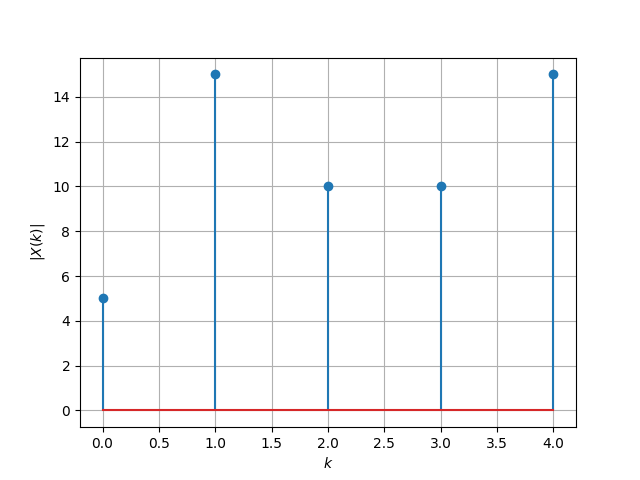
\includegraphics[width=\columnwidth]{2023/EC/47/figs/mm1.png}
    \caption{Amplitude of equation \eqref{eq:gate23ec47eq3}}
    \label{fig:gate23ec47fig1}
\end{figure}
\begin{figure}[htbp]
    \centering
    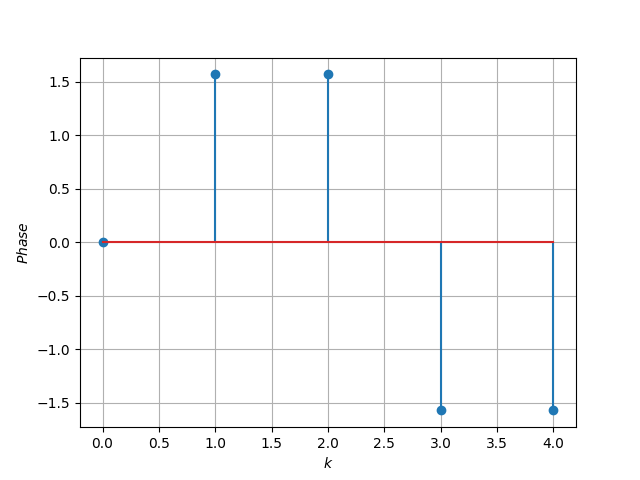
\includegraphics[width=\columnwidth]{2023/EC/47/figs/mm11.png}
    \caption{Phase of equation \eqref{eq:gate23ec47eq3}}
    \label{fig:gate23ec47fig2}
\end{figure}

\item Solving the question for N=8:
\begin{table}[h!]
 	\centering
 	\resizebox{6 cm}{!}{
 		\begin{tabular}{|c|c|c|}
    \hline
    \textbf{Parameter} & \textbf{Value} & \textbf{Description} \\[6pt]
    \hline
    $N$ &  $8$ & Time period \\ \cline{1-2}\cline{3-3}
    $X(k)$ &  $\sum\limits_{n=0}^{N-1} x(n)e^{\frac{-j2\pi kn}{N}}$ & DFT formula\\ \cline{1-2}\cline{3-3}
    $X(0)$ &  $8$ & \multirow{5}{*}{\begin{tabular}[c]{@{}c@{}}DFT \\ values\end{tabular}} \\ \cline{1-2}
    $X(1)$ &  $24j$ &    \\ \cline{1-2}
    $X(2)$ &  $16j$ &    \\ \cline{1-2}
    $X(3)$ &  $-16j$ &    \\ \cline{1-2}
    $X(4)$ &  $-24j$ &    \\ \cline{1-2}
    $X(5)$ &  $0$ &    \\ \cline{1-2}
    $X(6)$ &  $0$ &    \\ \cline{1-2}
    $X(7)$ &  $0$ &    \\ \hline
\end{tabular}

 	}
 	\vspace{6 pt}
 	\caption{Input Parameters}
 	\label{tab:gate23ec47tab1}
 \end{table} 
\begin{align}
\sum\limits_{n=0}^{7}x(n) \sin\brak{\frac{4\pi n}{8}}&=\sum\limits_{n=0}^{7}x(n)\sbrak{\frac{e^{\frac{j4\pi n}{8}}-e^{\frac{-j4\pi n}{8}}}{2j}}\\
&=\frac{1}{2j}\sbrak{\sum\limits_{n=0}^{7}x(n)e^{\frac{j2\pi (2)n}{8}}-\sum\limits_{n=0}^{7}x(n)e^{\frac{-j2\pi (2)n}{8}}}\label{eq:gate23ec47eq9}
\end{align}

Refering to the table \ref{tab:gate23ec47tab1}.
\begin{align}
X(k)&=\sum\limits_{n=0}^{7} x(n)e^{\frac{-j2\pi kn}{8}}\label{eq:gate23ec47eq10}
\end{align}
Referencing from equation\eqref{eq:gate23ec47eq10}, equation\eqref{eq:gate23ec47eq9} can be written as:
\begin{align}
\sum\limits_{n=0}^{7}x(n) \sin\brak{\frac{4\pi n}{8}}&=\frac{1}{2j}\sbrak{X(-2)-X(2)}\label{eq:gate23ec47eq11}
\end{align}
From the property of discrete Fourier series.\\
\begin{align}
X(k)=X(k+N)
\end{align}
So, equation\eqref{eq:gate23ec47eq11} becomes,\\
\begin{align}
\sum\limits_{n=0}^{7}x(n) \sin\brak{\frac{4\pi n}{8}}&=\frac{1}{2j}\sbrak{X(6)-X(2)}\\
\sum\limits_{n=0}^{7}x(n) \sin\brak{\frac{4\pi n}{8}}&=-8
\end{align}
\begin{figure}[h!]
    \centering
    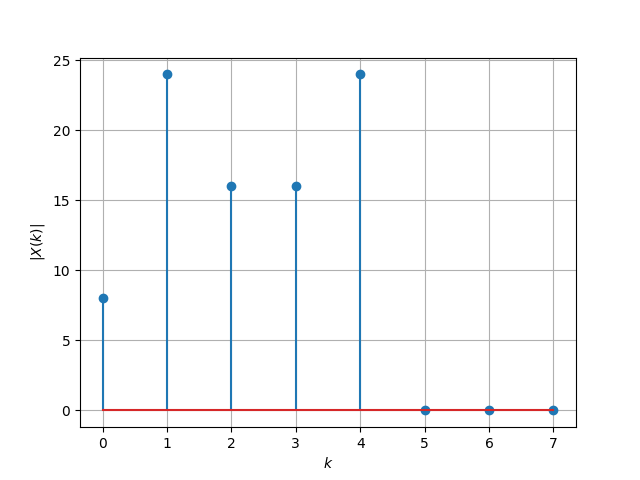
\includegraphics[width=\columnwidth]{2023/EC/47/figs/mm2.png}
    \caption{Amplitude of equation \eqref{eq:gate23ec47eq10}}
    \label{fig:gate23ec47fig3}
\end{figure}
\begin{figure}[h!]
    \centering
    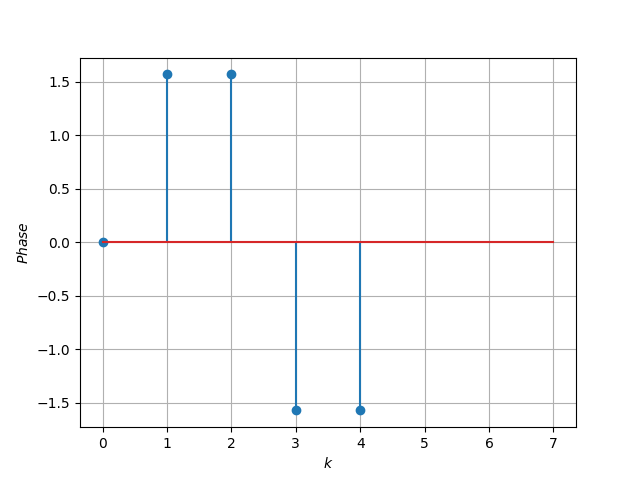
\includegraphics[width=\columnwidth]{2023/EC/47/figs/mm21.png}
    \caption{Phase of equation \eqref{eq:gate23ec47eq10}}
    \label{fig:gate23ec47fig4}
\end{figure}

\end{enumerate}

%\end{document}

\pagebreak

\item A continuous time, band-limited signal $x(t)$ has its Fourier transform described by:
\[ X(f) = \begin{cases} 
1 - \frac{|f|}{200} & \text{if } |f| \leq 200 \\
0 & \text{if } |f| > 200 
\end{cases} \]
The signal is uniformly sampled at a sampling rate of 600 Hz. The Fourier transform of the signal is $X_s(f)$. What is the value of $\frac{X_s(600)}{X_s(500)}$? \\\hfill{(GATE 2023 BM)}
\solution
\iffalse
\let\negmedspace\undefined
\let\negthickspace\undefined
\documentclass[journal,12pt,twocolumn]{IEEEtran}
\usepackage{cite}
\usepackage{amsmath,amssymb,amsfonts,amsthm}
\usepackage{algorithmic}
\usepackage{graphicx}
\usepackage{textcomp}
\usepackage{xcolor}
\usepackage{txfonts}
\usepackage{listings}
\usepackage{enumitem}
\usepackage{mathtools}
\usepackage{gensymb}
\usepackage{comment}
\usepackage[breaklinks=true]{hyperref}
\usepackage{tkz-euclide} 
\usepackage{listings}
\usepackage{gvv}                                        
\def\inputGnumericTable{}                                 
\usepackage[latin1]{inputenc}                                
\usepackage{color}                                            
\usepackage{array}                                            
\usepackage{longtable}                                       
\usepackage{calc}                                             
\usepackage{multirow}                                         
\usepackage{hhline}                                           
\usepackage{ifthen}                                           
\usepackage{lscape}


\newtheorem{theorem}{Theorem}[section]
\newtheorem{problem}{Problem}
\newtheorem{proposition}{Proposition}[section]
\newtheorem{lemma}{Lemma}[section]
\newtheorem{corollary}[theorem]{Corollary}
\newtheorem{example}{Example}[section]
\newtheorem{definition}[problem]{Definition}
\newcommand{\BEQA}{\begin{eqnarray}}
\newcommand{\EEQA}{\end{eqnarray}}
\newcommand{\define}{\stackrel{\triangle}{=}}
\theoremstyle{remark}
\newtheorem{rem}{Remark}
\begin{document}
\parindent 0px
\bibliographystyle{IEEEtran}

\title{Gate EE - 18}
\author{EE23BTECH11216 - P.kalyan$^{}$% <-this % stops a space
}
\maketitle
\newpage
\bigskip

\renewcommand{\thefigure}{\theenumi}
\renewcommand{\thetable}{\theenumi}
\section*{Question}
The Fourier transform x$\brak{\omega}$ of  the signal x\brak{t} is given by

\[
X(\omega) = 
\begin{cases} 
1, \text{for } |\omega| < \omega_0 \\
0, \text{for } |\omega| > \omega_0 
\end{cases}
\]

\text{(A) } x\brak{t} \text{ tends to be an impulse as } $W_0$ $\rightarrow \infty$.

\text{(B) } x\brak{0} \text{ decreases as } $W_0$ \text{ increases.}

\text{(C) At } t = $\frac{\pi}{2W_0}$, \quad x\brak{t} = -$\frac{1}{\pi}$.

\text{(D) At } t = $\frac{\pi}{2W_0}$, \quad x\brak{t} = $\frac{1}{\pi}$. \hfill\brak{\text{GATE EE 2023}}


 \fi

\begin{center}
    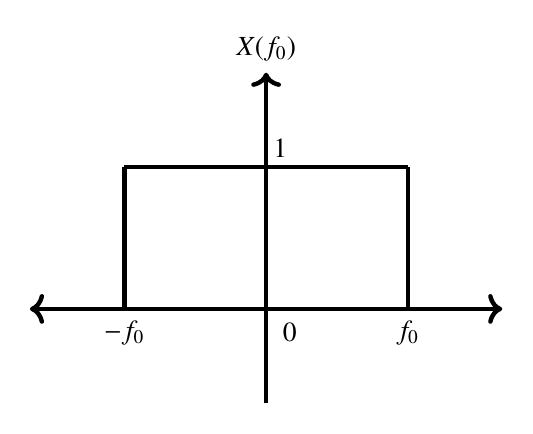
\begin{tikzpicture}[scale=0.6, ultra thick]
        \draw[->] (0,-2) -- (0,5);
        \draw (0,5.5) node {$X(f_{0}$)};
        \draw (0.5,-0.5)  node{0};
        \draw[<->]  (-5,0) -- (5,0);
        \draw  (3,3) -- (3,0);
        \draw (0.3,3.4) node{1};
        \draw (-3,3) -- (3,3);
        \draw (-3,3)--(-3,0);
        \draw (-3,-0.5) node {$-f_{0}$};

        \draw (3,-0.5) node {$f_{0}$};
    \end{tikzpicture}
\end{center}

By taking inverse Fourier transform,
\begin{align}
x\brak{t} = \frac{\sin\brak{ t}}{\pi t}
\end{align}

\begin{align}
& x\left(\frac{\pi}{2\brak{2\pi f_{0}}}\right) =\frac{2 \brak{2\pi f_{0}}}{\pi^2}
\end{align}

So, option \brak{C} and \brak{D} are wrong.

\begin{align}
x\brak{0}=\lim_{t\to 0}\frac{\sin \brak{2\pi f_{0}} t}{\pi t}=\frac{2\pi f_{0}}{\pi}
\end{align}

So, $x\brak{0} \propto f_{0} \Rightarrow$ Option \brak{B} is wrong.\\

When $f_{0}\rightarrow \infty$, $X\brak{f_{0}}$ will be a D.C signal and inverse Fourier transform of a D.C signal will be impulse signal\\[3ex]
So, option \brak{A} is correct
\begin{figure}[ht]
    \centering
    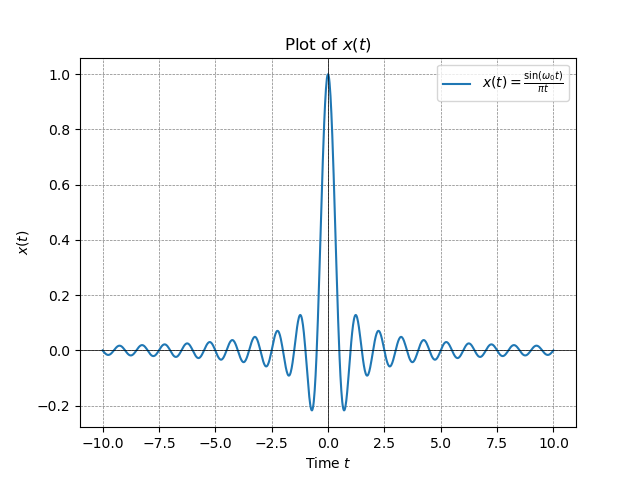
\includegraphics[width=1\columnwidth]{2023/EE/18/figs/main.png}
    \caption{plot of X\brak{t}}
    \label{fig:EE18.1}
\end{figure}


\pagebreak

 \item The magnitude and phase plots of an LTI systems are shown in figure. Find the transfer function.
\begin{figure}[!h]
    \centering
    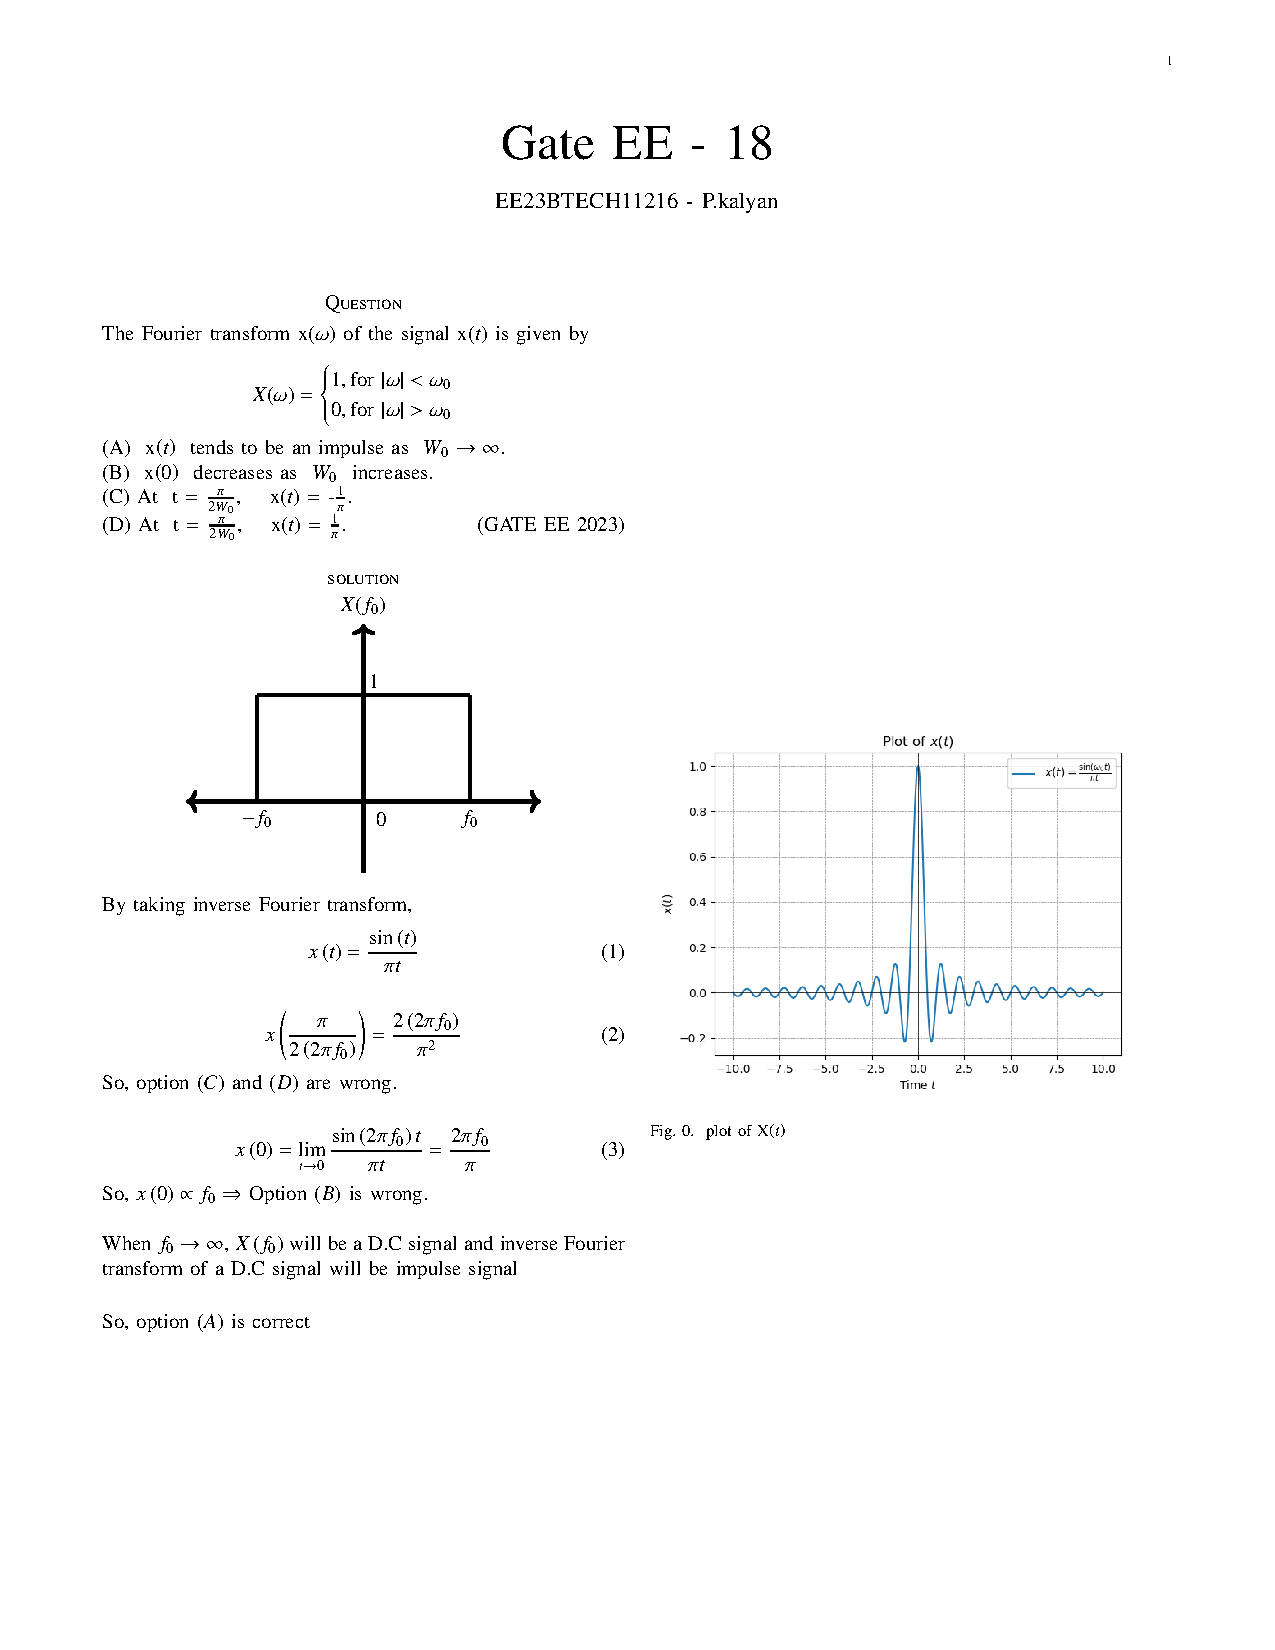
\includegraphics[width=\columnwidth]{2023/EE/36/figs/gate.png}
    \caption{}
    \label{fig:EEgatefig36.23}
\end{figure}
\begin{enumerate}
    \item $2.511 e^{-0.0032s}$\\
    \item $\frac{e^{-2.514s}}{s+1}$\\
    \item $1.04e^{-2.514s}$\\
    \item $2.511 e^{-1.047s}$\\
\end{enumerate} \hfill{(GATE EE 23)}\\

\solution
\input{2023/EE/36/36.tex}
\newpage
\item The value of the convolution of $f(x) = 3\cos(2x)$ and $g(x) = \frac{1}{3}\sin(2x)$ where $x \in [0, 2\pi)$, at $x = \frac{\pi}{3}$, is (Rounded off to 2 decimal places)\\
\hfill (GATE 2023 GE)\\
\solution
\input{2023/GE/81/ge.tex}
\pagebreak
\item A system is described by the following differential equation
    \[
    0.01 \frac{d^2y(t)}{dt^2} + 0.2\frac{dy(t)}{dt} + y(t) = 6x(t)
    \]
    where time \( t \) is in seconds. If \( x(t) \) is the unit step input applied at \( t = 0 \) s to this system, the magnitude of the output at \( t = 1 \) s is \(\underline{\hspace{2cm}}\). (Round off the answer to two decimal places.)
    \hfill (GATE-2023.BM)\\
    \solution
    \iffalse
\let\negmedspace\undefined
\let\negthickspace\undefined
\documentclass[journal,12pt,twocolumn]{IEEEtran}
\usepackage{cite}
\usepackage{amsmath,amssymb,amsfonts,amsthm}
\usepackage{algorithmic}
\usepackage{graphicx}
\usepackage{textcomp}
\usepackage{xcolor}
\usepackage{txfonts}
\usepackage{listings}
\usepackage{enumitem}
\usepackage{mathtools}
\usepackage{gensymb}
\usepackage{comment}
\usepackage[breaklinks=true]{adjustbox}
\usepackage{tkz-euclide} 
\usepackage{listings}
\usepackage{gvv}                                        
\def\inputGnumericTable{}                                 
\usepackage[latin1]{inputenc}                                
\usepackage{color}                                            
\usepackage{array}                                            
\usepackage{longtable}                                       
\usepackage{calc}                                             
\usepackage{multirow}                                         
\usepackage{hhline}                                           
\usepackage{ifthen}                                           
\usepackage{lscape}

\newtheorem{theorem}{Theorem}[section]
\newtheorem{problem}{Problem}
\newtheorem{proposition}{Proposition}[section]
\newtheorem{lemma}{Lemma}[section]
\newtheorem{corollary}[theorem]{Corollary}
\newtheorem{example}{Example}[section]
\newtheorem{definition}[problem]{Definition}
\newcommand{\BEQA}{\begin{eqnarray}}
\newcommand{\EEQA}{\end{eqnarray}}
\newcommand{\define}{\stackrel{\triangle}{=}}
\theoremstyle{remark}
\newtheorem{rem}{Remark}

\begin{document}
\bibliographystyle{IEEEtran}

\vspace{3cm}

\title{}
\author{EE23BTECH11024 - G.Karthik Yadav$^{*}$
}
\maketitle
\newpage
\bigskip

\section*{GATE 2023 EC 41}
\noindent 1. \hspace{2pt} A Closed loop systen is shown in the figure where $k>0$ and $\alpha>0$ .\\
The Steady State error due to a ramp input $\brak{R\brak{s} = \alpha s^{-2}}$ is given by \hfill{(GATE 2023 EC 41)}

\begin{figure}[ht]
\centering
    \includegraphics[width=1.0\linewidth]{2023/EC/41/figs/question.png}
    \label{fig: 23.EC.41.24.1}
\end{figure}

\begin{enumerate}
\item $\frac{2\alpha}{k}$
\item $\frac{\alpha}{k}$
\item $\frac{\alpha}{2k}$
\item $\frac{\alpha}{4k}$
\end{enumerate}

\solution\\
\fi
\begin{table}[ht]
\setlength{\arrayrulewidth}{0.3mm}
\setlength{\tabcolsep}{15pt}
\renewcommand{\arraystretch}{1.5}



\begin{tabular}{ |p{1cm}|p{3cm}|p{1cm}| }
\hline
Symbol & Parameters & Value\\
\hline
$R\brak{s}$ & Laplace transform Ramp input signal r\brak{t} &  $\alpha s^{-2}$\\
\hline
$G\brak{s}$ & Open Loop transfer function &  $ \frac{Y\brak{s}}{E\brak{s}} = \frac{k}{s\brak{s+2}}$\\
\hline
$Y\brak{s}$ & Laplace transform of the output signal y\brak{t}  &  ? \\
\hline
$E\brak{s}$ & Laplace transform of the error signal e\brak{t} & R\brak{s} - Y\brak{s}\\
\hline
$E\brak{s}$ & Laplace transform of the error signal e\brak{t} & R\brak{s} - Y\brak{s}\\   
\hline
$e_s$ & Steady State Error &  ? \\
\hline
%$x(l)$ & Last($l^{th}$) term of series & 350\\
%$x(0)$ & Starting ($0^{th}$) term of series & 17 %\\
%\hline
%d & Common difference of AP & 9\\
%\hline
\end{tabular}
\caption{Parameters}






\end{table}
\bigskip
from table  Open loop transfer function $G\brak{s}$\\
\begin{align}
	G\brak{s} &= \frac{Y\brak{s}}{E\brak{s}} \label{24.2023.EC.41.1} \\
        &= \frac{Y\brak{s}}{R\brak{s} - Y\brak{s}} \\
        Y\brak{s} &= \frac{R\brak{s}G\brak{s}}{1 + G\brak{s}} \label{24.2023.EC.41.2}
\end{align}

from eq \ref{24.2023.EC.41.1} and eq \eqref{24.2023.EC.41.2}

\begin{align}
        G\brak{s} &= \frac{k}{s\brak{s +2}}  \label{24.2023.EC.41.3} \\ 
        Y\brak{s} &= \frac{\alpha k s^{-2}}{k + s\brak{s+2}} \label{24.2023.EC.41.4} \\
        E\brak{s} &= R\brak{s} - Y\brak{s}  \label{24.2023.EC.41.5} \\ 
        E\brak{s} &= \frac{\alpha \brak{s+2}}{s\brak{k + s\brak{s+2}}}
\end{align}

By Taking Inverse Laplace Transform of eq \eqref{24.2023.EC.41.3} and eq\eqref{24.2023.EC.41.4}

\begin{align}
    g\brak{t} &= \frac{k\brak{1 - e^{-2t}}}{2} u\brak{t} \\
        y\brak{t} &= \alpha t u\brak{t}- \frac{2\alpha}{k}u\brak{t} \\
        \notag &+\frac{\alpha}{2k\sqrt{1-k}} \biggl(2\sqrt{1-k}e^{\sqrt{1-k}t-1}\\ 
        \notag &+ 2\sqrt{1-k}e^{-\sqrt{1-k}t-1} \\
        \notag &+ \brak{2-k}e^{\sqrt{1-k}t-1} - \brak{2-k}e^{-\sqrt{1-k}t-1} \biggr) u\brak{t}
\end{align}

\begin{align}
        e\brak{t} &= r\brak{t} - y\brak{t} \\
        &= \alpha t u\brak{t} - y\brak{t} \\
        e\brak{t} &= \frac{2\alpha}{k}u\brak{t} \\
        \notag &-\frac{\alpha}{2k\sqrt{1-k}} \biggl(2\sqrt{1-k}e^{\sqrt{1-k}t-1}\\ 
        \notag &+ 2\sqrt{1-k}e^{-\sqrt{1-k}t-1} \\
        \notag &+ \brak{2-k}e^{\sqrt{1-k}t-1} - \brak{2-k}e^{-\sqrt{1-k}t-1} \biggr) u\brak{t}
\end{align}
	

\begin{align}
    e_s &= \displaystyle\lim_{s\to 0}s E\brak{s} \\
    &= \displaystyle\lim_{s\to 0} s \frac{R\brak{s}}{1 + G\brak{s}} \\
    &= \displaystyle\lim_{s\to 0} \frac{\alpha \brak{s+2}}{s\brak{s+2} + k} \\
    e_s &= \frac{2\alpha}{k}
\end{align}



    \pagebreak

\item In the differential equation $\frac{dy}{dx} + \alpha x y = 0, \alpha$ is a positive constant. If $y = 1.0$ at
$x = 0.0$, and $y = 0.8$ at $x = 1.0$, the value of $\alpha$ is (rounded off to three decimal places).  \hfill(GATE CE 30 2023)\\
\solution
\iffalse
\let\negmedspace\undefined
\let\negthickspace\undefined
\documentclass[journal,12pt,twocolumn]{IEEEtran}
\usepackage{cite}
\usepackage{amsmath,amssymb,amsfonts,amsthm}
\usepackage{algorithmic}
\usepackage{graphicx}
\usepackage{textcomp}
\usepackage{xcolor}
\usepackage{txfonts}
\usepackage{listings}
\usepackage{enumitem}
\usepackage{mathtools}
\usepackage{gensymb}
\usepackage{comment}
\usepackage[breaklinks=true]{adjustbox}
\usepackage{tkz-euclide} 
\usepackage{listings}
\usepackage{gvv}                                        
\def\inputGnumericTable{}                                 
\usepackage[latin1]{inputenc}                                
\usepackage{color}                                            
\usepackage{array}                                            
\usepackage{longtable}                                       
\usepackage{calc}                                             
\usepackage{multirow}                                         
\usepackage{hhline}                                           
\usepackage{ifthen}                                           
\usepackage{lscape}

\newtheorem{theorem}{Theorem}[section]
\newtheorem{problem}{Problem}
\newtheorem{proposition}{Proposition}[section]
\newtheorem{lemma}{Lemma}[section]
\newtheorem{corollary}[theorem]{Corollary}
\newtheorem{example}{Example}[section]
\newtheorem{definition}[problem]{Definition}
\newcommand{\BEQA}{\begin{eqnarray}}
\newcommand{\EEQA}{\end{eqnarray}}
\newcommand{\define}{\stackrel{\triangle}{=}}
\theoremstyle{remark}
\newtheorem{rem}{Remark}

\begin{document}
\bibliographystyle{IEEEtran}

\vspace{3cm}

\title{}
\author{EE23BTECH11024 - G.Karthik Yadav$^{*}$
}
\maketitle
\newpage
\bigskip

\section*{GATE 2023 EC 41}
\noindent 1. \hspace{2pt} A Closed loop systen is shown in the figure where $k>0$ and $\alpha>0$ .\\
The Steady State error due to a ramp input $\brak{R\brak{s} = \alpha s^{-2}}$ is given by \hfill{(GATE 2023 EC 41)}

\begin{figure}[ht]
\centering
    \includegraphics[width=1.0\linewidth]{2023/EC/41/figs/question.png}
    \label{fig: 23.EC.41.24.1}
\end{figure}

\begin{enumerate}
\item $\frac{2\alpha}{k}$
\item $\frac{\alpha}{k}$
\item $\frac{\alpha}{2k}$
\item $\frac{\alpha}{4k}$
\end{enumerate}

\solution\\
\fi
\begin{table}[ht]
\setlength{\arrayrulewidth}{0.3mm}
\setlength{\tabcolsep}{15pt}
\renewcommand{\arraystretch}{1.5}



\begin{tabular}{ |p{1cm}|p{3cm}|p{1cm}| }
\hline
Symbol & Parameters & Value\\
\hline
$R\brak{s}$ & Laplace transform Ramp input signal r\brak{t} &  $\alpha s^{-2}$\\
\hline
$G\brak{s}$ & Open Loop transfer function &  $ \frac{Y\brak{s}}{E\brak{s}} = \frac{k}{s\brak{s+2}}$\\
\hline
$Y\brak{s}$ & Laplace transform of the output signal y\brak{t}  &  ? \\
\hline
$E\brak{s}$ & Laplace transform of the error signal e\brak{t} & R\brak{s} - Y\brak{s}\\
\hline
$E\brak{s}$ & Laplace transform of the error signal e\brak{t} & R\brak{s} - Y\brak{s}\\   
\hline
$e_s$ & Steady State Error &  ? \\
\hline
%$x(l)$ & Last($l^{th}$) term of series & 350\\
%$x(0)$ & Starting ($0^{th}$) term of series & 17 %\\
%\hline
%d & Common difference of AP & 9\\
%\hline
\end{tabular}
\caption{Parameters}






\end{table}
\bigskip
from table  Open loop transfer function $G\brak{s}$\\
\begin{align}
	G\brak{s} &= \frac{Y\brak{s}}{E\brak{s}} \label{24.2023.EC.41.1} \\
        &= \frac{Y\brak{s}}{R\brak{s} - Y\brak{s}} \\
        Y\brak{s} &= \frac{R\brak{s}G\brak{s}}{1 + G\brak{s}} \label{24.2023.EC.41.2}
\end{align}

from eq \ref{24.2023.EC.41.1} and eq \eqref{24.2023.EC.41.2}

\begin{align}
        G\brak{s} &= \frac{k}{s\brak{s +2}}  \label{24.2023.EC.41.3} \\ 
        Y\brak{s} &= \frac{\alpha k s^{-2}}{k + s\brak{s+2}} \label{24.2023.EC.41.4} \\
        E\brak{s} &= R\brak{s} - Y\brak{s}  \label{24.2023.EC.41.5} \\ 
        E\brak{s} &= \frac{\alpha \brak{s+2}}{s\brak{k + s\brak{s+2}}}
\end{align}

By Taking Inverse Laplace Transform of eq \eqref{24.2023.EC.41.3} and eq\eqref{24.2023.EC.41.4}

\begin{align}
    g\brak{t} &= \frac{k\brak{1 - e^{-2t}}}{2} u\brak{t} \\
        y\brak{t} &= \alpha t u\brak{t}- \frac{2\alpha}{k}u\brak{t} \\
        \notag &+\frac{\alpha}{2k\sqrt{1-k}} \biggl(2\sqrt{1-k}e^{\sqrt{1-k}t-1}\\ 
        \notag &+ 2\sqrt{1-k}e^{-\sqrt{1-k}t-1} \\
        \notag &+ \brak{2-k}e^{\sqrt{1-k}t-1} - \brak{2-k}e^{-\sqrt{1-k}t-1} \biggr) u\brak{t}
\end{align}

\begin{align}
        e\brak{t} &= r\brak{t} - y\brak{t} \\
        &= \alpha t u\brak{t} - y\brak{t} \\
        e\brak{t} &= \frac{2\alpha}{k}u\brak{t} \\
        \notag &-\frac{\alpha}{2k\sqrt{1-k}} \biggl(2\sqrt{1-k}e^{\sqrt{1-k}t-1}\\ 
        \notag &+ 2\sqrt{1-k}e^{-\sqrt{1-k}t-1} \\
        \notag &+ \brak{2-k}e^{\sqrt{1-k}t-1} - \brak{2-k}e^{-\sqrt{1-k}t-1} \biggr) u\brak{t}
\end{align}
	

\begin{align}
    e_s &= \displaystyle\lim_{s\to 0}s E\brak{s} \\
    &= \displaystyle\lim_{s\to 0} s \frac{R\brak{s}}{1 + G\brak{s}} \\
    &= \displaystyle\lim_{s\to 0} \frac{\alpha \brak{s+2}}{s\brak{s+2} + k} \\
    e_s &= \frac{2\alpha}{k}
\end{align}



\pagebreak

\end{enumerate}
